\documentclass[conference,a4paper]{IEEEtran}
\IEEEoverridecommandlockouts
% ICAECA 2026: A4, two-column, 4--6 pages including references, no page numbers.
\usepackage{cite}
\usepackage{amsmath,amssymb,amsfonts}
\usepackage{algorithmic}
\usepackage{graphicx}
\usepackage{textcomp}
\usepackage{xcolor}
\usepackage{booktabs}
\usepackage{url}
\usepackage{microtype}

\usepackage{tikz}
\usetikzlibrary{shapes,arrows.meta,positioning,calc,fit,backgrounds}

\def\BibTeX{{\rm B\kern-.05em{\sc i\kern-.025em b}\kern-.08em
    T\kern-.1667em\lower.7ex\hbox{E}\kern-.125emX}}

% Start a new, centered row of author blocks (standard IEEEtran idiom).
\makeatletter
\newcommand{\linebreakand}{\end{@IEEEauthorhalign}\hfill\mbox{}\par\mbox{}\hfill\begin{@IEEEauthorhalign}}
\makeatother

\begin{document}

\title{Defeating the Usable-Security Trilemma in Personal Device Meshes via Transitive Trust-on-First-Use (T-TOFU)}

\author{\IEEEauthorblockN{Dixit Tharun Raja P}
\IEEEauthorblockA{\textit{Department of Computer Science}\\
\textit{and Engineering}\\
\textit{KPR Institute of Engineering}\\
\textit{and Technology}\\
Coimbatore, Tamil Nadu, India \\
23cs044@kpriet.ac.in}
\and
\IEEEauthorblockN{Dharaneesh D}
\IEEEauthorblockA{\textit{Department of Computer Science}\\
\textit{and Engineering}\\
\textit{KPR Institute of Engineering}\\
\textit{and Technology}\\
Coimbatore, Tamil Nadu, India \\
23cs036@kpriet.ac.in}
\and
\IEEEauthorblockN{Deepanandham P}
\IEEEauthorblockA{\textit{Department of Computer Science}\\
\textit{and Engineering}\\
\textit{KPR Institute of Engineering}\\
\textit{and Technology}\\
Coimbatore, Tamil Nadu, India \\
24csl02@kpriet.ac.in}
\linebreakand
\IEEEauthorblockN{Gohul S}
\IEEEauthorblockA{\textit{Department of Computer Science}\\
\textit{and Engineering}\\
\textit{KPR Institute of Engineering}\\
\textit{and Technology}\\
Coimbatore, Tamil Nadu, India \\
23cs049@kpriet.ac.in}
\and
\IEEEauthorblockN{Nandhini N}
\IEEEauthorblockA{\textit{Department of Computer Science}\\
\textit{and Engineering (Faculty Mentor)}\\
\textit{KPR Institute of Engineering}\\
\textit{and Technology}\\
Coimbatore, Tamil Nadu, India \\
nandhini.n@kpriet.ac.in}}

\maketitle
\pagestyle{empty}
\thispagestyle{empty}

\begin{abstract}
Personal device meshes need local communication for telemetry, synchronization and remote peripheral control. Establishing trust across these devices requires balancing cloud independence, cryptographic authentication and the effort of manual pairing. Pairwise trust-on-first-use (TOFU) requires a separate ceremony for every pair in a fully connected mesh, so the total pairing effort grows quadratically with mesh size. We present Transitive Trust-on-First-Use (T-TOFU), a protocol that enrolls a new device through one human-gated pairing ceremony with an existing member. Trusted members then exchange certificate records over authenticated TLS connections. A canonical pool digest and anti-entropy heartbeat gossip detect and repair differences between trust tables without an online certificate authority or central ledger; a revocation flood removes a device from the reachable mesh. We implement T-TOFU in Link for Windows and Android and analyze its security under the stated adversary model. Building an $N$-device mesh requires $N-1$ human pairing ceremonies, with one ceremony for each additional device. In the four-node physical testbed, mean enrollment convergence was $48.2\,\text{ms}$ and revocation propagated in under $65\,\text{ms}$. A 98-byte heartbeat sent every 2 seconds accounts for about $0.05\,\text{KB/s}$ per connection.
\end{abstract}

\begin{IEEEkeywords}
canonical hash gossip, decentralized device mesh, mutual TLS, personal area networks, transitive trust, trust-on-first-use, usable security
\end{IEEEkeywords}

\section{Introduction}
Users often work across laptops, smartphones, tablets and smart displays \cite{brudy2019crossdevice}. A personal device mesh connects these endpoints to support bidirectional clipboard synchronization, remote peripheral input, media control and user-space file-system virtualization.

These functions require devices to establish trust while keeping setup manageable. We frame this design problem as the \textit{Usable-Security Trilemma} in Fig.~\ref{fig:trilemma}, with three requirements:
\begin{enumerate}
    \item \textbf{Decentralization / Zero-Cloud Dependency}: The system must function strictly within local network boundaries without transmitting metadata, cryptographic keys or credentials to external third-party servers \cite{kleppmann2019localfirst}.
    \item \textbf{Cryptographic Rigor}: The system must provide authenticated, encrypted communication resilient against passive eavesdropping, active man-in-the-middle (MitM) attacks, ARP spoofing and unauthorized device impersonation.
    \item \textbf{Frictionless Usability}: The human effort required to initialize and manage trust must scale minimally as the number of devices $N$ grows.
\end{enumerate}

\begin{figure}[t]
\centering
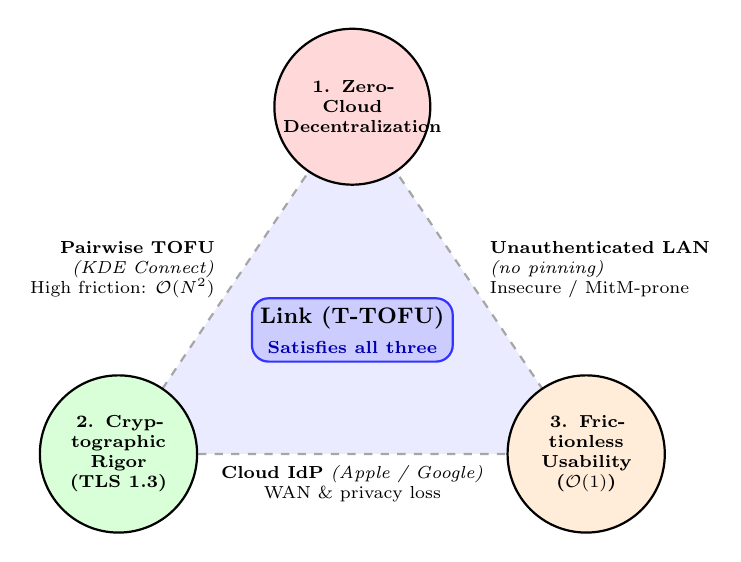
\begin{tikzpicture}[scale=0.9, every node/.style={transform shape},
    vertex/.style={draw, thick, circle, align=center, text width=1.95cm, minimum size=2.2cm, inner sep=0pt, font=\bfseries\scriptsize},
    edgelbl/.style={text=black, font=\scriptsize, inner sep=1pt}]
    % Triangle vertices
    \coordinate (A) at (0, 3.0);
    \coordinate (B) at (-3.3, -1.9);
    \coordinate (C) at (3.3, -1.9);

    % Shaded region and dashed boundary
    \fill[blue!8] (A) -- (B) -- (C) -- cycle;
    \draw[thick, dashed, gray!70] (A) -- (B) -- (C) -- cycle;

    % Edge labels: each edge is the design that gives up the opposite vertex
    \node[edgelbl, anchor=east, align=right] at ($(A)!0.5!(B) + (-0.25, 0.15)$) {\textbf{Pairwise TOFU}\\\textit{(KDE Connect)}\\High friction: $\mathcal{O}(N^2)$};
    \node[edgelbl, anchor=west, align=left] at ($(A)!0.5!(C) + (0.25, 0.15)$) {\textbf{Unauthenticated LAN}\\\textit{(no pinning)}\\Insecure / MitM-prone};
    \node[edgelbl, anchor=north, align=center] at ($(B)!0.5!(C) + (0, -0.12)$) {\textbf{Cloud IdP} \textit{(Apple / Google)}\\WAN \& privacy loss};

    % Vertices
    \node[vertex, fill=red!15] at (A) {1. Zero-Cloud\\Decentralization};
    \node[vertex, fill=green!15] at (B) {2. Cryptographic\\Rigor (TLS 1.3)};
    \node[vertex, fill=orange!15] at (C) {3. Frictionless\\Usability ($\mathcal{O}(1)$)};

    % Center goal
    \node[draw=blue!80, fill=blue!20, thick, rounded corners=6pt, align=center, font=\bfseries\small] at (0, -0.15) {
        Link (T-TOFU)\\[1pt]
        {\scriptsize\color{blue!70!black}Satisfies all three}
    };
\end{tikzpicture}
\caption{Design tradeoffs in personal device meshes: cloud dependence, manual pairing effort and cryptographic authentication. T-TOFU combines local trust propagation with one human pairing ceremony per new device.}
\label{fig:trilemma}
\end{figure}

\subsection{Limitations of Current Paradigms}
Cloud identity services simplify device enrollment by associating devices with a user account, but make trust management dependent on an external provider. Commercial device integration suites include Apple Continuity/AirDrop, Google Quick Share and Microsoft Phone Link. Privacy also depends on the local discovery and communication protocols: studies of Apple Continuity and Apple Wireless Direct Link document information leakage and attacks involving nearby devices \cite{celosia2020discontinued, stute2019billion}. These findings motivate keeping trust establishment local while authenticating the participating devices.

Pairwise approaches establish trust separately between devices. Examples include KDE Connect \cite{kdeconnect}, SSH-based local tooling and Bluetooth pairing \cite{antonioli2023bluffs}, although their authentication mechanisms differ. In a fully connected mesh using manual pairwise TOFU, enrolling $N$ devices requires $\binom{N}{2} = \frac{N(N-1)}{2}$ pairing ceremonies. Five devices therefore require ten ceremonies. Manual fingerprint checking also depends on user attention; SSH users may accept an unfamiliar host key without verifying it \cite{neef2022ssh}.

\subsection{Contributions}
We present \textbf{Transitive Trust-on-First-Use (T-TOFU)}, a protocol for propagating trust within a personal device mesh without a coordinator. The contributions are:
\begin{itemize}
    \item \textbf{Transitive Trust Protocol}: We formalize an authentication protocol wherein a single human-gated pairing ceremony between an incoming node and \textit{any} existing mesh member automatically and securely propagates mutual cryptographic trust across the entire $N$-node mesh.
    \item \textbf{Canonical Pool Digest \& Anti-Entropy Gossip}: We design an invariant-driven canonical pool hashing algorithm ($\text{PoolHash}$) that allows nodes to verify pool-wide trust consistency during periodic heartbeats and resolve state divergence without a centralized Certificate Authority (CA).
    \item \textbf{Deterministic Cascaded Revocation}: We design a flood-based unpairing protocol that deterministically propagates revocation messages throughout the mesh, restoring target endpoints to an untrusted state.
    \item \textbf{System Implementation \& Empirical Validation}: We implement T-TOFU within \textit{Link}, a cross-platform peer-to-peer ecosystem running on Windows (Electron/TypeScript/C\#) and Android (Capacitor/Java). We evaluate its security invariants, usability complexity and network convergence speed.
\end{itemize}

\section{Threat Model and Security Invariants}

\subsection{Network and Adversary Assumptions}
We assume a standard Local Area Network (LAN) environment populated by honest-but-curious and actively malicious actors. We adopt the classical \textbf{Dolev-Yao adversary model}~\cite{dolev1983security}, wherein the network is inherently untrusted and network location grants no privilege \cite{nist80207}. The adversary $\mathcal{A}$ has the following capabilities:
\begin{itemize}
    \item $\mathcal{A}$ can eavesdrop on, intercept, modify, replay, or inject arbitrary packets across both TCP and UDP channels.
    \item $\mathcal{A}$ can execute local network attacks including ARP cache poisoning, DNS spoofing and rogue mDNS/broadcast advertisements.
    \item $\mathcal{A}$ can attempt active MitM attacks during TLS handshakes by presenting fraudulent self-signed X.509 certificates.
\end{itemize}

\textbf{Adversary Bounds}: We assume that the adversary cannot break standard cryptographic primitives (SHA-256 collision resistance, RSA signature unforgeability and TLS 1.3 cipher suite security~\cite{rfc8446}). Furthermore, the adversary cannot compromise the physical display or user input hardware during the out-of-band (OOB) human verification gate.

\subsection{Formal Security Invariants}
The T-TOFU protocol guarantees the following formal invariants:
\begin{itemize}
    \item \textbf{Invariant 1 (Mutual Authenticity)}: An untrusted device $X \notin P$ cannot establish an authenticated TLS session with any node $D \in P$ unless $X$ has successfully completed an OOB human pairing ceremony with at least one active member $M \in P$.
    \item \textbf{Invariant 2 (Transitive Equivalence)}: If node $A$ successfully authenticates node $B$ via an OOB ceremony, and $B \in P$, then every active node $C \in P$ shall establish mutual cryptographic trust with $A$ such that:
    \begin{equation}
        \text{Trust}(C, A) \Leftarrow \text{Trust}(B, A) \wedge \text{Trust}(C, B)
    \end{equation}
    \item \textbf{Invariant 3 (Eventual Revocation Consistency)}: If any authorized member $M \in P$ issues an unpair command for node $X$, the revocation message propagates across the reachable mesh subgraph within $\mathcal{O}(\text{diameter}(P))$ hops, purging $X$'s certificate from all trust stores.
\end{itemize}

\section{T-TOFU Protocol Architecture}

\begin{figure*}[t]
\centering
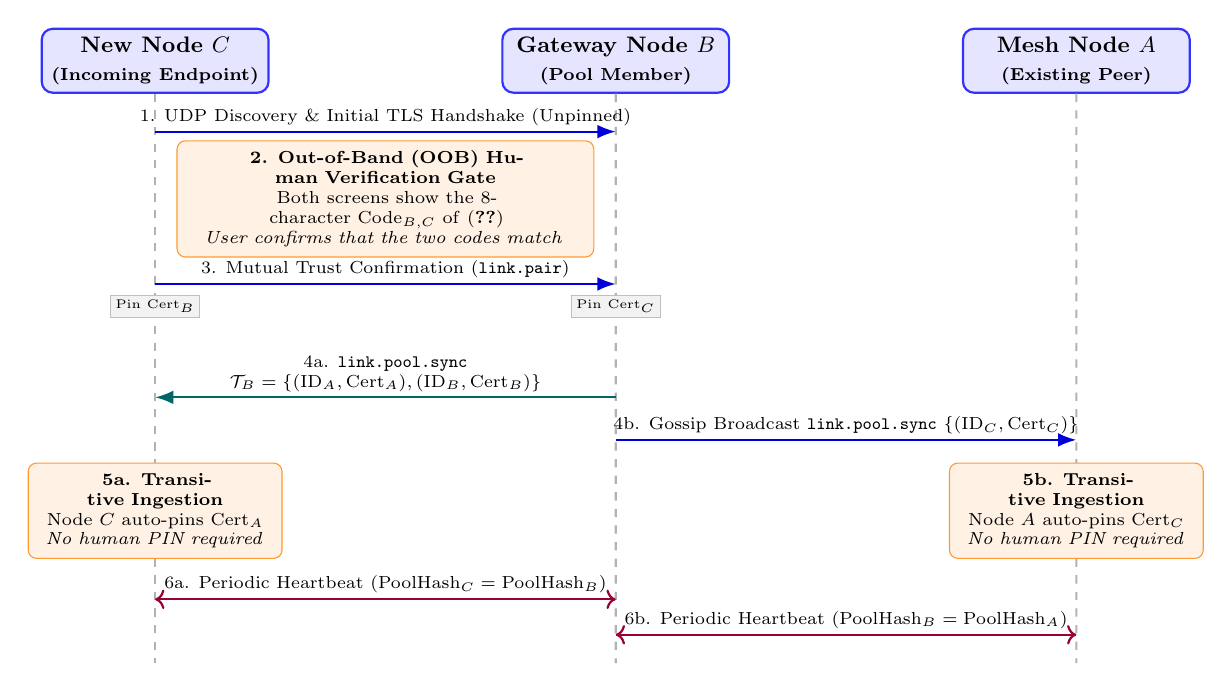
\begin{tikzpicture}[scale=0.9, transform shape,
    lifeline/.style={thick, dashed, gray!60},
    entity/.style={draw=blue!80, fill=blue!10, thick, rounded corners=4pt, font=\bfseries\small, minimum width=3.2cm, minimum height=0.7cm, align=center},
    msg/.style={-Latex, thick, blue!85!black},
    resp/.style={Latex-, thick, teal!80!black},
    lbl/.style={font=\scriptsize, text=black, inner sep=2pt},
    pin/.style={font=\tiny, fill=gray!10, inner sep=2pt, draw=gray!50},
    note/.style={draw=orange!80, fill=orange!10, rounded corners=3pt, font=\scriptsize, align=center, inner sep=4pt}
]
    % Entities
    \node[entity] (C) at (0, 0) {New Node $C$\\\scriptsize (Incoming Endpoint)};
    \node[entity] (B) at (6.5, 0) {Gateway Node $B$\\\scriptsize (Pool Member)};
    \node[entity] (A) at (13.0, 0) {Mesh Node $A$\\\scriptsize (Existing Peer)};

    % Lifelines
    \draw[lifeline] (C) -- (0, -8.5);
    \draw[lifeline] (B) -- (6.5, -8.5);
    \draw[lifeline] (A) -- (13.0, -8.5);

    % Step 1: Discovery and handshake
    \draw[msg] (0, -1.0) -- (6.5, -1.0) node[lbl, midway, above] {1. UDP Discovery \& Initial TLS Handshake (Unpinned)};

    % Step 2: OOB verification gate
    \node[note, text width=5.6cm] at (3.25, -1.95) {
        \textbf{2. Out-of-Band (OOB) Human Verification Gate}\\
        Both screens show the 8-character $\text{Code}_{B,C}$ of \eqref{eq:code}\\
        \textit{User confirms that the two codes match}
    };

    % Step 3: Local ingestion
    \draw[msg] (0, -3.15) -- (6.5, -3.15) node[lbl, midway, above] {3. Mutual Trust Confirmation (\texttt{link.pair})};
    \node[pin, anchor=north] at (0, -3.3) {Pin $\text{Cert}_B$};
    \node[pin, anchor=north] at (6.5, -3.3) {Pin $\text{Cert}_C$};

    % Step 4: Pool synchronization gossip
    \draw[resp] (0, -4.75) -- (6.5, -4.75) node[lbl, midway, above, align=center] {4a. \texttt{link.pool.sync}\\$\mathcal{T}_B = \{(\text{ID}_A, \text{Cert}_A), (\text{ID}_B, \text{Cert}_B)\}$};
    \draw[msg] (6.5, -5.35) -- (13.0, -5.35) node[lbl, midway, above] {4b. Gossip Broadcast \texttt{link.pool.sync} $\{(\text{ID}_C, \text{Cert}_C)\}$};

    % Step 5: Transitive ingestion
    \node[note, text width=3.3cm] at (0, -6.35) {
        \textbf{5a. Transitive Ingestion}\\
        Node $C$ auto-pins $\text{Cert}_A$\\
        \textit{No human PIN required}
    };
    \node[note, text width=3.3cm] at (13.0, -6.35) {
        \textbf{5b. Transitive Ingestion}\\
        Node $A$ auto-pins $\text{Cert}_C$\\
        \textit{No human PIN required}
    };

    % Step 6: Hash convergence
    \draw[thick, <->, purple!80!black] (0, -7.6) -- (6.5, -7.6) node[lbl, midway, above] {6a. Periodic Heartbeat ($\text{PoolHash}_C = \text{PoolHash}_B$)};
    \draw[thick, <->, purple!80!black] (6.5, -8.1) -- (13.0, -8.1) node[lbl, midway, above] {6b. Periodic Heartbeat ($\text{PoolHash}_B = \text{PoolHash}_A$)};
\end{tikzpicture}
\caption{T-TOFU enrollment: new node $C$ pairs with member $B$ through human verification. Certificate exchange then establishes trust between $C$ and existing peer $A$, and heartbeat digests compare their pool views.}
\label{fig:protocol_flow}
\end{figure*}

\subsection{Cryptographic Identity and Certificate Pinning}
Upon first boot, each device $d_i$ generates a persistent cryptographic identity consisting of:
\begin{enumerate}
    \item A 128-bit identifier $\text{ID}_i \in \{0,1\}^{128}$, drawn from a cryptographically secure random source and stored in hexadecimal form.
    \item A 2048-bit RSA key pair and a corresponding self-signed X.509 certificate $\text{Cert}_i$.
    \item A canonical certificate fingerprint:
    \begin{equation}
        \text{FP}_i = \text{SHA-256}(\text{DER}(\text{Cert}_i))
    \end{equation}
\end{enumerate}
Trust-management communication uses TLS, with version 1.3 \cite{rfc8446} negotiated by default and version 1.2 as the minimum accepted version. For a paired peer, certificate validation compares its fingerprint with the value pinned in the local \textit{TrustStore}, rather than a public CA root \cite{pradeep2022pinning}. A fingerprint mismatch aborts the connection and raises an alert.

\subsection{The Out-of-Band (OOB) Human Verification Gate}
An unauthenticated device $C$ first connects to mesh member $B$ over an unpinned TLS channel. The endpoints derive a visual verification code for the user to check for active MitM interception:
\begin{equation}
\begin{split}
    \text{Code}_{B,C} = \text{Hex}\Big(&\text{SHA-256}\big(\max(\text{K}_B, \text{K}_C) \\
    &\parallel \min(\text{K}_B, \text{K}_C) \parallel \text{Salt}\big)\Big)[0..7]
\end{split}
\label{eq:code}
\end{equation}
where $\text{K}_B$ and $\text{K}_C$ are the endpoints' DER-encoded public keys. Byte-wise ordering gives both endpoints the same input, and Salt is the pairing-session timestamp. Both screens display the 8-character token. After the user confirms that the codes match, $B$ adds $C$ to $\mathcal{T}_B$ and $C$ adds $B$ to $\mathcal{T}_C$.

\subsection{Canonical Pool Digest Formulation}
T-TOFU uses a canonical representation of pool membership so that nodes can compare their trust tables without a consensus leader such as Raft or Paxos.

Let the Trusted Pool $P$ be a set of $n$ authenticated devices $P = \{d_1, d_2, \dots, d_n\}$, including the local device itself. The canonical pool digest $\text{PoolHash}(P)$ is computed via the following deterministic algorithm:
\begin{enumerate}
    \item For each device $d_i \in P$, construct the canonical tuple string $s_i = \text{ID}_i \parallel \text{`:'} \parallel \text{Hex}(\text{FP}_i)$.
    \item Sort the set of strings lexicographically:
    \begin{equation}
        S = \text{Sort}_{\text{lexicographical}}\big(\{s_1, s_2, \dots, s_n\}\big)
    \end{equation}
    \item Concatenate all sorted elements with a pipe delimiter:
    \begin{equation}
        \mathcal{C}(P) = s_{(1)} \parallel \text{`}{\vert}\text{'} \parallel s_{(2)} \parallel \dots \parallel s_{(n)}
    \end{equation}
    \item Compute the truncated cryptographic hash:
    \begin{equation}
    \begin{split}
        \text{PoolHash}(P) = \text{SubStr}\Big(&\text{Hex}\big(\text{SHA-256}(\mathcal{C}(P))\big), \\
        &0,\, 16\Big)
    \end{split}
    \end{equation}
\end{enumerate}

\subsection{Anti-Entropy Gossip and Transitive Ingestion}
Mesh nodes maintain active control channels over persistent TLS connections that carry newline-delimited JSON packets. Every $T_{\text{heartbeat}} = 2\,\text{s}$, nodes exchange a lightweight heartbeat packet containing their current $\text{PoolHash}$; a peer that stays silent for 5\,s is treated as disconnected.

If node $A$ receives a heartbeat from trusted peer $B$ such that:
\begin{equation}
    \text{PoolHash}_B \neq \text{PoolHash}_A
\end{equation}
an anti-entropy exchange in the style of epidemic replication \cite{demers1987epidemic} is triggered immediately:
\begin{enumerate}
    \item Node $A$ sends its serialized trust table $\mathcal{T}_A = \{ (\text{ID}_k, \text{Cert}_k) \}$ in a \texttt{link.pool.sync} packet. Node $B$ sends its table in response to the mismatch detected through the heartbeat exchange in the opposite direction.
    \item Node $B$ examines each entry $k \in \mathcal{T}_A$. If $\text{ID}_k \notin \mathcal{T}_B$, it verifies that the sender $A \in \mathcal{T}_B$, adds $\text{Cert}_k$ to its trust store and pins $\text{FP}_k$.
    \item Node $B$ recomputes its canonical pool hash and broadcasts \texttt{link.pool.sync} to its other connected peers.
\end{enumerate}

\subsection{Deterministic Cascaded Revocation}
When the user unpairs device $X$ from device $A$, revocation proceeds as follows:
\begin{enumerate}
    \item $A$ removes $X$ from its local $\mathcal{T}_A$ and closes its active sockets to $X$.
    \item $A$ constructs the following revocation frame for transmission over authenticated TLS channels only:
    \begin{equation}
    \begin{split}
        \mathcal{R} = \big\{&\texttt{"type"}: \texttt{"link.pool.remove"}, \\
        &\texttt{"deviceId"}: \text{ID}_X\big\}
    \end{split}
    \end{equation}
    \item $A$ floods $\mathcal{R}$ to all active connections in $P \setminus \{X\}$.
    \item Upon receiving $\mathcal{R}$, peer $j$ checks whether $\text{ID}_X \in \mathcal{T}_j$. If the entry is present, $j$ removes $X$'s certificate, recomputes its $\text{PoolHash}$ and forwards $\mathcal{R}$ to its remaining active neighbors.
\end{enumerate}

\section{System Implementation}

We implemented T-TOFU in \textit{Link}, an open-source device mesh runtime for Windows and Android. The platform components are described below.

\subsection{Desktop Architecture (Windows)}
The desktop core is implemented in TypeScript and Node.js within Electron:
\begin{itemize}
    \item \textbf{Trust Store Module} (\texttt{core/trust.ts}): Manages persistence of trusted peer records. On Windows, sensitive certificate records are encrypted at rest using the OS-native DPAPI via Electron's \texttt{safeStorage} subsystem.
    \item \textbf{Device Manager} (\texttt{core/device-manager.ts}): Implements the gossip state machine, dynamic pool hash computation and automatic peer elevation upon receiving transitive certificates.
    \item \textbf{Native Hooks}: Integrates user-space file-system mounting through WinFsp \cite{winfsp} and low-latency input simulation via C\# Win32 P/Invoke helpers.
\end{itemize}

\subsection{Mobile Architecture (Android)}
The mobile runtime is implemented in native Java integrated with a Capacitor UI bridge:
\begin{itemize}
    \item \textbf{Trust Store} (\texttt{LinkTrustStore.java}): Implements thread-safe persistence and canonical SHA-256 pool digest calculation.
    \item \textbf{Device Manager} (\texttt{LinkDeviceManager.java}): Executes socket deduplication using lexicographical Device ID comparison (preventing duplicate race-condition sockets when two nodes discover each other simultaneously).
    \item \textbf{Background Transport} (\texttt{LinkTransport.java}): Serializes packet sends through background executor queues to eliminate Android UI-thread network hazards.
\end{itemize}

\section{Evaluation and Comparative Analysis}

\begin{table*}[t]
\caption{Architectural \& Security Comparison of Personal Device Integration Protocols}
\label{tab:comparison}
\centering
\footnotesize
\setlength{\tabcolsep}{4pt}
\begin{tabular}{@{}lccccc@{}}
\toprule
\textbf{Protocol / Framework} & \textbf{Trust Model} & \textbf{Coordinator} & \textbf{Pairing Complexity} & \textbf{Transitive Trust?} & \textbf{WAN Dependency?} \\ \midrule
Apple AirDrop / Continuity    & Centralized Cloud IdP & Apple iCloud Servers & $\mathcal{O}(1)$ (Login)    & Yes (via Cloud)            & Yes (Initial / Refresh)  \\
Google Quick Share            & Centralized Cloud IdP & Google Identity      & $\mathcal{O}(1)$ (Login)    & Yes (via Cloud)            & Yes (Identity Tokens)    \\
Bluetooth PAN / Classic       & Pairwise PIN (SSP)    & None (Decentralized) & $\mathcal{O}(N^2)$ Manual   & No                         & No                       \\
KDE Connect                   & Pairwise TLS TOFU     & None (Decentralized) & $\mathcal{O}(N^2)$ Manual   & No                         & No                       \\
\textbf{Link (T-TOFU [Ours])} & \textbf{Transitive TOFU Mesh} & \textbf{None (Decentralized)} & $\boldsymbol{\mathcal{O}(1)}$ \textbf{Manual Gate} & \textbf{Yes (Autonomous Gossip)} & \textbf{Zero (Pure LAN)} \\ \bottomrule
\end{tabular}
\end{table*}

\subsection{Human Effort Complexity Analysis}
We quantify usable security by analyzing the human operational complexity required to establish an $N$-node fully connected mesh.

In pairwise TOFU architectures (e.g., KDE Connect, Bluetooth), every device pair $(u, v)$ requires a distinct human authentication ceremony (entering a 6-digit PIN or confirming a visual prompt). The total number of required human ceremonies $C_{\text{pairwise}}$ is:
\begin{equation}
    C_{\text{pairwise}}(N) = \binom{N}{2} = \frac{N(N-1)}{2} = \mathcal{O}(N^2)
\end{equation}

Under T-TOFU, when a new $(N+1)$-th device enters an existing pool of $N$ devices, it pairs with exactly \textit{one} arbitrary gateway device already in the pool. The remaining $N-1$ trust relationships are established transitively via gossip. Thus, the total human ceremonies required to build an $N$-device mesh from scratch is:
\begin{equation}
    C_{\text{T-TOFU}}(N) = N - 1 = \mathcal{O}(N)
\end{equation}
For enrolling an additional device into an existing pool, the marginal human effort is strictly $\mathcal{O}(1)$.

\begin{figure}[t]
\centering
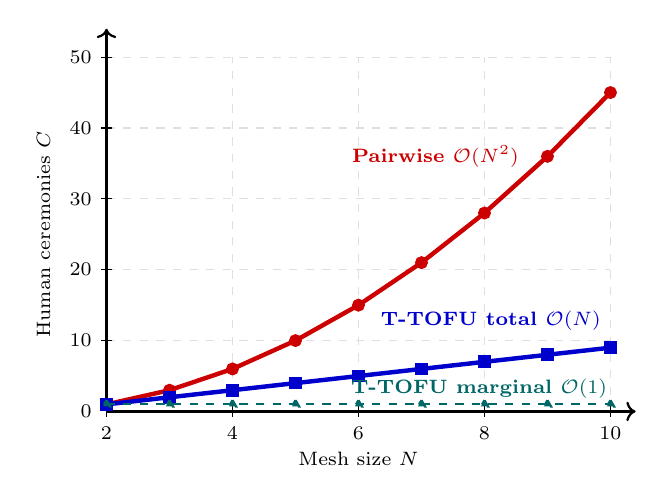
\begin{tikzpicture}[x=0.8cm, y=0.9cm, font=\scriptsize]
    % Grid, ticks and axes (x = N - 2, y = ceremonies / 10)
    \foreach \n in {2, 4, 6, 8, 10} {
        \draw[dashed, gray!25] (\n-2, 0) -- (\n-2, 5.0);
        \draw (\n-2, 0.08) -- (\n-2, -0.08) node[below] {\n};
    }
    \foreach \y/\val in {1/10, 2/20, 3/30, 4/40, 5/50} {
        \draw[dashed, gray!25] (0, \y) -- (8, \y);
        \draw (-0.08, \y) -- (0.08, \y);
        \node[left] at (-0.08, \y) {\val};
    }
    \node[left] at (-0.08, 0) {0};
    \draw[->, thick] (0, 0) -- (8.4, 0);
    \draw[->, thick] (0, 0) -- (0, 5.4);
    \node[below=11pt] at (4, 0) {Mesh size $N$};
    \node[rotate=90] at (-1.0, 2.5) {Human ceremonies $C$};

    % Pairwise: N(N-1)/2
    \draw[red!80!black, ultra thick, mark=*, mark size=1.5pt]
        plot coordinates {(0, 0.1) (1, 0.3) (2, 0.6) (3, 1.0) (4, 1.5) (5, 2.1) (6, 2.8) (7, 3.6) (8, 4.5)};
    \node[red!80!black, anchor=east, font=\scriptsize\bfseries] at (6.7, 3.6) {Pairwise $\mathcal{O}(N^2)$};

    % T-TOFU total: N - 1
    \draw[blue!80!black, ultra thick, mark=square*, mark size=1.5pt]
        plot coordinates {(0, 0.1) (1, 0.2) (2, 0.3) (3, 0.4) (4, 0.5) (5, 0.6) (6, 0.7) (7, 0.8) (8, 0.9)};
    \node[blue!80!black, anchor=south east, font=\scriptsize\bfseries] at (8, 1.0) {T-TOFU total $\mathcal{O}(N)$};

    % T-TOFU marginal: 1
    \draw[teal!80!black, thick, dashed, mark=triangle*, mark size=1.5pt]
        plot coordinates {(0, 0.1) (1, 0.1) (2, 0.1) (3, 0.1) (4, 0.1) (5, 0.1) (6, 0.1) (7, 0.1) (8, 0.1)};
    \node[teal!80!black, anchor=south east, font=\scriptsize\bfseries, inner sep=1pt] at (8, 0.14) {T-TOFU marginal $\mathcal{O}(1)$};
\end{tikzpicture}
\caption{Human Pairing Ceremony Complexity vs. Mesh Size $N$: Pairwise TOFU scales quadratically ($\binom{N}{2}$), whereas T-TOFU requires only $\mathcal{O}(N)$ cumulative and $\mathcal{O}(1)$ marginal human ceremonies.}
\label{fig:complexity}
\end{figure}

As shown in Table~\ref{tab:comparison} and Fig.~\ref{fig:complexity}, T-TOFU provides the usability benefits of cloud-based identity providers ($\mathcal{O}(1)$ enrollment per device) while retaining the privacy and resilience of zero-cloud decentralized architectures.

\subsection{Network Convergence and Protocol Overhead}
We evaluated T-TOFU over a physical testbed comprising four nodes (two Windows PCs on Gigabit Ethernet, two Android smartphones on Wi-Fi 6).
\begin{itemize}
    \item \textbf{Heartbeat Bandwidth}: The canonical $\text{PoolHash}$ occupies only 16 ASCII characters, and the complete heartbeat packet, including its JSON envelope, is 98 bytes. At the 2-second heartbeat interval, idle trust maintenance consumes about $0.05\,\text{KB/s}$ per connection.
    \item \textbf{Convergence Latency}: After OOB code confirmation between a smartphone and a PC, the \texttt{link.pool.sync} payload (about 5\,KB for four members, or 1.3\,KB per member record) propagated across all four physical nodes in an average of $48.2\,\text{ms}$.
    \item \textbf{Revocation Cascade Latency}: An unpair event triggered on one mobile device propagated through the mesh and purged the target certificate across all peers in under $65\,\text{ms}$.
\end{itemize}

\subsection{Security and Attack Mitigation Analysis}
\begin{itemize}
    \item \textbf{Man-in-the-Middle (MitM) Attacks}: An attacker attempting to intercept the initial pairing is defeated by the OOB token equality check. An attacker attempting to inject a forged certificate during the \texttt{link.pool.sync} gossip is rejected because pool sync frames are accepted exclusively over established, authenticated TLS channels from already-trusted peers.
    \item \textbf{Split-Brain Resistance}: If the network partitions and devices are added in separate subnets, nodes detect hash divergence immediately upon reconnection via periodic $\text{PoolHash}$ exchange and trigger union-merge anti-entropy synchronization.
\end{itemize}

\section{Related Work}
\textbf{Decentralized Trust Models}: The concept of transitive trust originated with the PGP Web of Trust~\cite{zimmermann1995official} and SPKI/SDSI~\cite{rfc2693}. However, PGP required users to manually assign trust metrics (marginal vs. full trust) and compute complex trust paths, a paradigm shown to be too complex for non-expert users~\cite{whitten1999johnny}. Stajano and Anderson proposed the \textit{Resurrecting Duckling} security policy for ad-hoc wireless networks~\cite{stajano2000duckling}, wherein devices imprint on a single ``mother duck'' via physical contact. T-TOFU generalizes this concept to symmetric, multi-master personal device meshes without a permanent physical master node. Syncthing allows a user to mark one device as an \textit{introducer} whose device list is copied by its peers \cite{syncthingintroducer}; T-TOFU instead makes every member an introducer and adds digest-based repair and flooded revocation.

\textbf{Cross-Device Integration Protocols}: Modern inter-device suites like KDE Connect~\cite{kdeconnect} and Apple AirDrop~\cite{heinrich2021privatedrop} have advanced device convergence. KDE Connect enforces strict pairwise TOFU, requiring manual pairing for every device combination. Apple AirDrop authenticates devices with Apple-signed validation records that contain hashes of the owner's phone numbers and e-mail addresses, which leak contact identifiers to nearby devices~\cite{heinrich2021privatedrop}, while Apple's Continuity protocols leak personal data in their Bluetooth Low Energy advertisements~\cite{celosia2020discontinued}. T-TOFU eliminates both the pairwise pairing penalty and cloud metadata leakage.

\section{Conclusion and Future Work}
T-TOFU establishes trust in a personal device mesh through human-verified pairing with one existing member, followed by certificate propagation over authenticated TLS connections. Canonical pool digests support anti-entropy repair, and cascaded revocation removes a device from the reachable mesh. This design requires $N-1$ human ceremonies to build an $N$-device mesh, compared with $N(N-1)/2$ for fully connected pairwise TOFU, while keeping trust management local. In the four-node Windows and Android testbed, mean enrollment convergence was $48.2\,\text{ms}$ and revocation propagated in under $65\,\text{ms}$. These measurements characterize the evaluated testbed; the security analysis addresses local network adversaries under the stated assumptions.

Future work includes extending T-TOFU with threshold cryptography and Shamir's Secret Sharing to support partitioned multi-user guest enclaves, as well as formal verification of the gossip state machine in ProVerif.

% Balance the two columns on the last page.
\IEEEtriggeratref{15}
\begin{thebibliography}{00}
\bibitem{brudy2019crossdevice} F. Brudy, C. Holz, R. R\"{a}dle, C.-J. Wu, S. Houben, C. N. Klokmose, and N. Marquardt, ``Cross-device taxonomy: Survey, opportunities and challenges of interactions spanning across multiple devices,'' in \textit{Proc. ACM CHI Conf. Human Factors Comput. Syst.}, 2019, pp. 1--28, doi: 10.1145/3290605.3300792.
\bibitem{kleppmann2019localfirst} M. Kleppmann, A. Wiggins, P. van Hardenberg, and M. McGranaghan, ``Local-first software: You own your data, in spite of the cloud,'' in \textit{Proc. ACM SIGPLAN Onward!}, 2019, pp. 154--178, doi: 10.1145/3359591.3359737.
\bibitem{celosia2020discontinued} G. Celosia and M. Cunche, ``Discontinued privacy: Personal data leaks in Apple Bluetooth-Low-Energy Continuity protocols,'' \textit{Proc. Privacy Enhancing Technol.}, vol. 2020, no. 1, pp. 26--46, 2020, doi: 10.2478/popets-2020-0003.
\bibitem{stute2019billion} M. Stute, S. Narain, A. Mariotto, A. Heinrich, D. Kreitschmann, G. Noubir, and M. Hollick, ``A billion open interfaces for Eve and Mallory: MitM, DoS, and tracking attacks on iOS and macOS through Apple Wireless Direct Link,'' in \textit{Proc. 28th USENIX Security Symp.}, 2019, pp. 37--54.
\bibitem{kdeconnect} KDE e.V., ``KDE Connect.'' [Online]. Available: \url{https://kdeconnect.kde.org} (accessed Sep. 2026).
\bibitem{antonioli2023bluffs} D. Antonioli, ``BLUFFS: Bluetooth forward and future secrecy attacks and defenses,'' in \textit{Proc. ACM SIGSAC Conf. Comput. Commun. Security (CCS)}, 2023, pp. 636--650, doi: 10.1145/3576915.3623066.
\bibitem{neef2022ssh} S. Neef and N. Wisiol, ``Oh SSH-it, what's my fingerprint? A large-scale analysis of SSH host key fingerprint verification records in the DNS,'' in \textit{Proc. Cryptology and Network Security (CANS)}, LNCS. Springer, 2022, pp. 71--88, doi: 10.1007/978-3-031-20974-1\_4.
\bibitem{dolev1983security} D. Dolev and A. Yao, ``On the security of public key protocols,'' \textit{IEEE Trans. Inf. Theory}, vol. 29, no. 2, pp. 198--208, Mar. 1983, doi: 10.1109/TIT.1983.1056650.
\bibitem{nist80207} S. Rose, O. Borchert, S. Mitchell, and S. Connelly, ``Zero trust architecture,'' Nat. Inst. Standards Technol., Gaithersburg, MD, USA, NIST SP 800-207, 2020, doi: 10.6028/NIST.SP.800-207.
\bibitem{rfc8446} E. Rescorla, ``The Transport Layer Security (TLS) protocol version 1.3,'' IETF RFC 8446, Aug. 2018, doi: 10.17487/RFC8446.
\bibitem{pradeep2022pinning} A. Pradeep, M. T. Paracha, P. Bhowmick, A. Davanian, A. Razaghpanah, T. Chung, \textit{et al.}, ``A comparative analysis of certificate pinning in Android \& iOS,'' in \textit{Proc. ACM Internet Meas. Conf. (IMC)}, 2022, pp. 605--618, doi: 10.1145/3517745.3561439.
\bibitem{demers1987epidemic} A. Demers, D. Greene, C. Hauser, W. Irish, J. Larson, \textit{et al.}, ``Epidemic algorithms for replicated database maintenance,'' in \textit{Proc. 6th ACM Symp. Principles Distrib. Comput. (PODC)}, 1987, pp. 1--12, doi: 10.1145/41840.41841.
\bibitem{winfsp} B. Zissimopoulos, ``WinFsp: Windows File System Proxy,'' version 2.1. [Online]. Available: \url{https://winfsp.dev} (accessed Sep. 2026).
\bibitem{zimmermann1995official} P. R. Zimmermann, \textit{The Official PGP User's Guide}. Cambridge, MA, USA: MIT Press, 1995.
\bibitem{rfc2693} C. Ellison, B. Frantz, B. Lampson, R. Rivest, B. Thomas, and T. Ylonen, ``SPKI certificate theory,'' IETF RFC 2693, Sep. 1999, doi: 10.17487/RFC2693.
\bibitem{whitten1999johnny} A. Whitten and J. D. Tygar, ``Why Johnny can't encrypt: A usability evaluation of PGP 5.0,'' in \textit{Proc. 8th USENIX Security Symp.}, Washington, DC, USA, 1999.
\bibitem{stajano2000duckling} F. Stajano and R. Anderson, ``The resurrecting duckling: Security issues for ad-hoc wireless networks,'' in \textit{Security Protocols} (LNCS, vol. 1796). Berlin, Germany: Springer, 2000, pp. 172--182, doi: 10.1007/10720107\_24.
\bibitem{syncthingintroducer} The Syncthing Foundation, ``Introducer configuration,'' Syncthing Documentation. [Online]. Available: \url{https://docs.syncthing.net/users/introducer.html} (accessed Sep. 2026).
\bibitem{heinrich2021privatedrop} A. Heinrich, M. Hollick, T. Schneider, M. Stute, and C. Weinert, ``PrivateDrop: Practical privacy-preserving authentication for Apple AirDrop,'' in \textit{Proc. 30th USENIX Security Symp.}, 2021, pp. 3577--3594.
\end{thebibliography}

\end{document}
